\documentclass[11pt, twoside, a4paper]{report}

\usepackage{float}

\usepackage{verbatim}
\usepackage{tikz}
\usetikzlibrary{arrows,shapes}
\tikzstyle{vertex} = [circle, fill=black!25, minimum size=100pt, inner sep=0pt]
\tikzstyle{edge} = [draw, thick, line width=1.5pt, inner sep=5pt, outer sep=5pt]

\begin{document}

\title{\textbf{Perceiving and memorising packaged goods} \\ (in a supermarket environment) \\ \vspace{7.5mm} \textsc{Diploma Thesis}}
\author{Carsten K\"onemann \\ \texttt{cargath@gmail.com}}
\date{08.10.2013}

\maketitle

\chapter{Abstract}

\tableofcontents

\chapter{Introduction}

\section{Review}
Current solutions can be divided into two groups: Those which search for a specific object as needed, and those which utilize a set of predetermined locations. \\

A solution which searches for an object as needed is much more flexible. Because such a system does not specify fixed locations for potential targets, it is able to find an object almost anywhere in its domain and is able to deal with objects that might change their location. It can adapted quickly by changing some simple assumptions about its domain. A housekeeping robot that is able to fetch a black coffee mug from a kitchen for example should also be able to fetch a white coffee mug from a living room after modifying a few parameters.

The downside to this approach is, that the search for an object requires time. The larger the search area, the longer a search takes and quickly becomes the most time consuming part of the task. Therefor this method is only applicable for small domains. \\

The second group is an approach often used for storage facilities and similar applications: A large warehouse, for example, which is organised in a way that all items have their specific place at which they can be found. When an agent is required to get an object, it does not need to perform a search first, because it already knows where to go.

While this is vastly superior for time critical use-cases, it is also a very unflexible approach that requires a complex setup, previous knowledge about the domain and high maintenance whenever something about the domain changes.

\section{Motivation / Goal} % "Das Ziel dieser Arbeit" - gutes Wort fuer "Arbeit" in Englisch?
The goal of this paper is to create a method combining the strengths of both of these popular current solutions. A flexible system which by itself maintains a dynamic memory about its environment and utilizes this knowledge in order to identify the nearest location with the highest certainty of an object requested by the user. \\

In order to accomplish this goal, the system uses a database of potentially interesting objects and basic information required to identify these objects. It continuesly does a basic processing of the stream of an agents camera image, without interfering with the agents current task. The camera image is only investigated further, when this basic processing gives reason to believe that one or more potentially interesting objects are visible. If further investigation confirms that a potentially interesting object has successfully been recognized, then its position and orientation are memorized in a semantic map. A user then is able to ask the system for an object it needs and receive a list of those that are most relevant in the current situation, i.e. evaluated by distance to the agents location and probability to still find the object where it was perceived.

\section{Scenario}
The system will be tested and presented in a shopping scenario, where an agent (e.g. a robot) is supposed to find objects from a shopping list in a supermarket. \\

A shopping scenario is a good example to illustrate the benefits of the method proposed in this paper, because a supermarket does arrange goods by grouping them by category and keeps using roughly the same place for a group over longer periods of time, but it does not provide a list of specific locations for third-parties to use to locate objects. Maintaining a list of locations for a shopping robot manually would require a lot of work, because supermarkets tend to switch things around slightly. \\

Since perceiving arbitrary objects is a whole field of study on its own this paper will focus on packaged supermarket goods, which is sufficient in the context of this scenario as well as for the purpose of demonstrating the method at hand.

\section{Structure}
%TODO


\newpage
\chapter{Methods}

\section{Architecture} % 'Echtes' UML verwenden?

\newpage
\begin{figure}[H]
  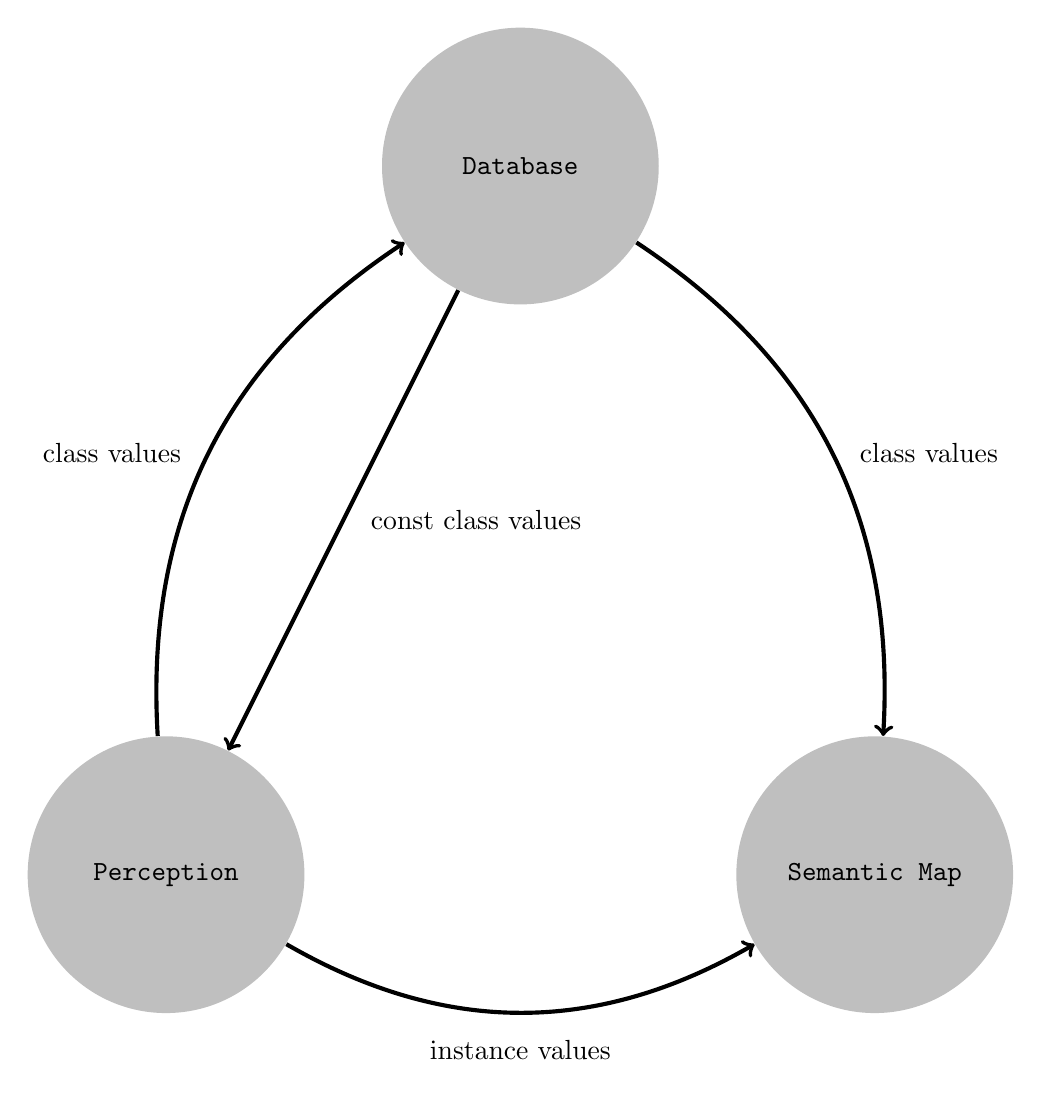
\begin{tikzpicture}[->, scale=1.8, auto, swap]
    % Draw the vertices.
    \node [vertex] (a) at (2.5, 5) {\texttt{Database}};
    \node [vertex] (b) at (  0, 0) {\texttt{Perception}};
    \node [vertex] (c) at (  5, 0) {\texttt{Semantic Map}};
    % Database <-> Perception.
    \path [edge] (a) edge [] node [right] {const class values} (b);
    \path [edge] (b) edge [bend left] node [left] {class values} (a);
    % Perception -> Semantic Map.
    \path [edge] (b) edge [bend right] node {instance values} (c);
    % Database -> Semantic Map.
    \path [edge] (a) edge [bend left] node [right] {class values} (c);
  \end{tikzpicture}
\end{figure}

\newpage
\subsection{Datatypes}
\subsection{Database}
\subsection{Perception}
\subsection{Semantic Map}
\subsection{Visualization}

\newpage
\section{Implementation}
\subsection{ROS}
\subsection{OpenCV}
\subsection{SiftGPU}
\subsection{PR2}
\subsection{RGB-D SLAM}
\subsection{Shared Library}
\subsection{Setup Samples}
\subsection{Mipmapping}
\subsection{Feature Detection and Matching}
\subsection{Filter Matches}
\subsection{Filter False Positives}
\subsection{Calculate 3D Pose}
\subsection{Memorise only new Objects}
\subsection{Evaluation Function}
\subsection{Tests}


\chapter{Analysis}
\section{Experimentation}
\section{Results}
\section{Evaluation}


\chapter{Discussion}


\chapter{Conclusion}


\chapter{Future Work / Outlook}


\end{document}
